\Microsoft \Azure Storage is a cloud storage system that provides customers the ability to store seemingly limitless amounts of data. It has grown from tens of petabytes in 2010 to exabytes in 2015, with the total number of objects stored well-exceeding 60 trillion.
%~\cite{greenberg2015keynote}.

\Azure Storage vNext is the next generation storage system for \Microsoft \Azure, where the primary design target is to scale the storage capacity by more than 100$\times$. Similar to the current system, vNext employs containers, called \emph{extents}, to store data. Extents are typically several gigabytes each, consisting of many data blocks, and replicated over multiple \emph{Extent Nodes} (ENs). However, in contrast to the current system, which employs a Paxos-based, centralized mapping from extents to ENs, vNext achieves its scalability target by employing a \emph{distributed mapping}. In vNext, extents are divided into partitions, with each partition managed by a light-weight \emph{Extent Manager} (ExtMgr). This partitioning is illustrated in Figure~\ref{fig:vnext}.

\begin{figure}[t]
\centering
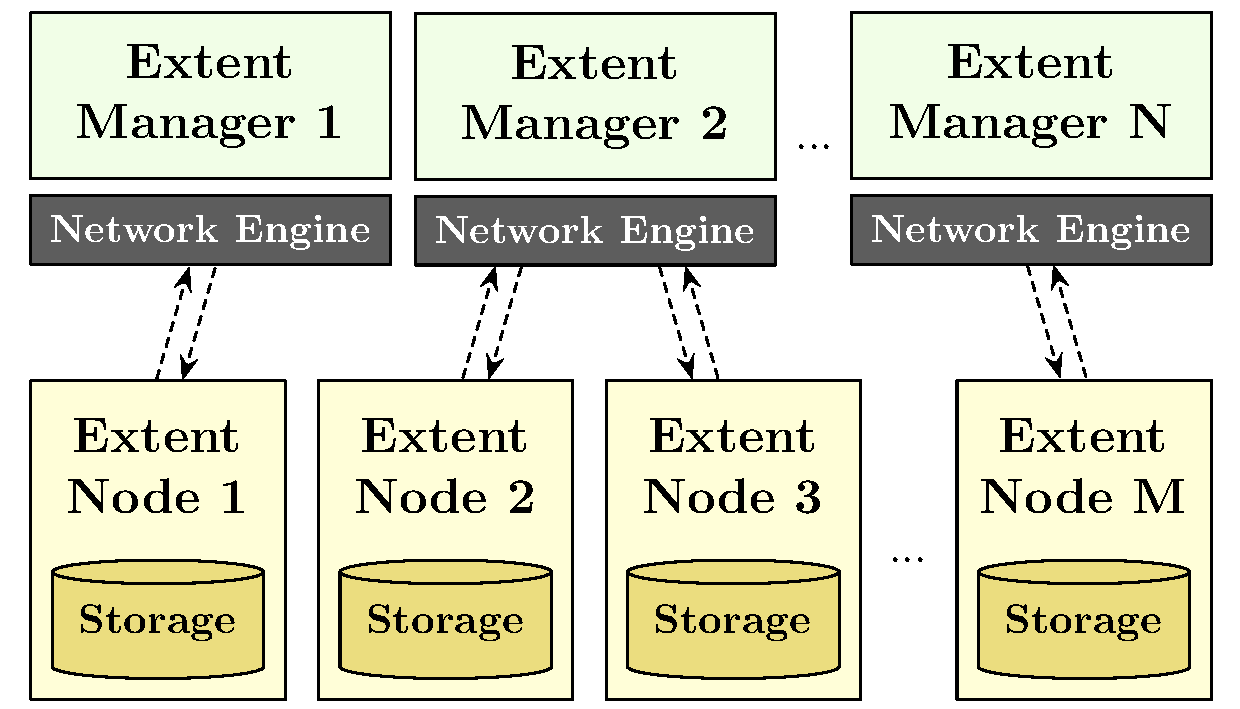
\includegraphics[width=\linewidth]{img/azurestore}
\caption{Top-level components for extent management in \Microsoft \Azure Storage vNext.}
\label{fig:vnext}
\end{figure}

One of the many responsibilities of an ExtMgr is to ensure that every extent maintains enough \emph{replicas} in the system. To achieve this, an ExtMgr receives frequent periodic \emph{heartbeat} messages from every EN. The failure of an EN is detected by missing heartbeats. An ExtMgr also receives less frequent, but still periodic, \emph{synchronization reports} from every EN. The sync reports list all the extents (and associated metadata) stored on the EN. Based on these two types of messages, an ExtMgr identifies which ENs have failed, and which extents are affected by the failure and are missing replicas as a result. The ExtMgr then schedules tasks to repair the affected extents and distributes the tasks to the necessary ENs. The ENs then repair the extents from their existing replicas in the system and lazily update the ExtMgr via their next periodic sync reports. All this communication between an ExtMgr and the ENs occurs via network engines installed in each component of vNext (see Figure~\ref{fig:vnext}).

To ensure correctness, the developers of vNext have instrumented extensive, multiple levels of testing:
\begin{enumerate}
\item \emph{Unit testing}, in which emulated heartbeats and sync reports are sent to an ExtMgr. These tests check that the messages are processed as expected.

\item \emph{Integration testing}, in which an ExtMgr is launched together with multiple ENs. An EN failure is subsequently injected. These tests check that the affected extents are eventually repaired.

\item \emph{Stress testing}, in which an ExtMgr is launched together with multiple ENs and multiple extents. The test keeps repeating the following process: injecting an EN failure, launching a new EN and checking that the affected extents are eventually repaired.
\end{enumerate}

\noindent
Despite of the extensive testing efforts, the vNext developers have been plagued for months by an elusive bug in the ExtMgr logic. All the unit test suites and integration test suites successfully pass every single time. However, the stress test suite fails \emph{from time to time} after very long executions; in these cases, certain replicas of some extents fail and are never repaired.

This bug has proven to be difficult to identify, reproduce and troubleshoot. First, an extent never being repaired is \emph{not} a property that can be easily checked. Second, the bug seems to manifest only in very long executions. Finally, by the time that the bug is detected, very long execution traces have been collected, which makes manual inspection tedious and ineffective. To uncover this bug, as well as many other tricky bugs, the vNext developers are in constant search of a generic and systematic approach for testing distributed systems.
